\documentclass[tikz,border=3.14mm]{standalone}
\usepackage{pgfplots}
\pgfplotsset{compat=1.16,width=16cm}
\tikzset{
	declare function={
		torusx(\u,\v,\R)=cos(\u)*(\R + cos(\v));
		torusy(\u,\v,\R)=(\R + cos(\v))*sin(\u);
		torusz(\u,\v,\R)=sin(\v);
}}
\begin{document}
	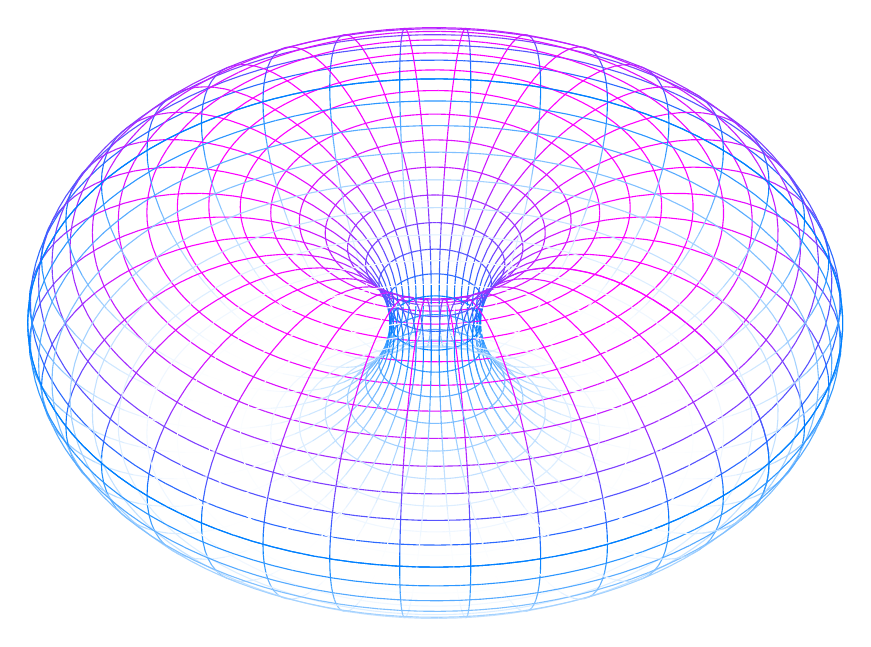
\begin{tikzpicture}
		\pgfmathsetmacro{\R}{1.25} % Major radius
		\pgfplotsset{view={35}{60},axis lines=none,}
		\begin{axis}[colormap/cool]
			% Generate the fluctuating torus mesh
			\pgfplotsinvokeforeach{0,10,...,360} {
				\addplot3[
				samples y=0,
				domain=0:360,
				smooth,
				samples=120,
				thin,
				mesh
				]  
				(
				{torusx(x,#1,\R)}, 
				{torusy(x,#1,\R)}, 
				{torusz(x,#1,\R)}
				);
				\addplot3[
				samples y=0,
				domain=0:360,
				smooth,
				samples=71,
				thin,
				mesh
				]  
				(
				{torusx(#1,x,\R)}, 
				{torusy(#1,x,\R)}, 
				{torusz(#1,x,\R)}
				);
			}
		\end{axis}
	\end{tikzpicture}
\end{document}
